%!TEX root=../robocert.tex
\begin{figure}[htb]
	\centering
	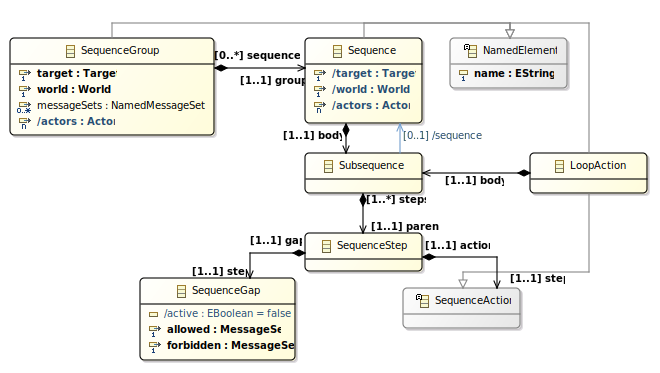
\includegraphics[width=\textwidth]{diagrams/Sequences}
	\caption{Class diagram for the part of the \langname{} metamodel dealing with sequences.}
	\label{fig:metamodel-sequences}
\end{figure}

The main tool for specifying properties of \robochart{} models in
\langname{} is \emph{sequences}.  These are diagrams, similar to UML2
sequence diagrams~\cite{lima-semantics} and Property Sequence Charts~\cite{psc},
that capture one or more valid traces of a robotic system.

\Cref{fig:metamodel-sequences} depicts the part of the metamodel concerning
sequence groups and sequences.

\subsection{\msequencegroup}

A \msequencegroup{} is a top-level \mnamedelement{} that contains sequence diagrams.
It contains:

\begin{itemize}
\item
  two \mactor s (\cref{sec:metamodel-actors}):
  a \mtarget{} (\cref{ssec:metamodel-actors-target})
  and a \mworld{} (\cref{ssec:metamodel-actors-world});
\item
  zero or more \mnamedmessageset{}s (\cref{ssec:metamodel-messages-named-sets});
\item
  zero or more \msequence{} (\cref{ssec:metamodel-sequences-sequences}).
\end{itemize}

\begin{lstlisting}[style=Example]
sequence group Group:
  module AModule  // RCModuleTarget actor
  -> world        // World actor
{
  message set M1: universe
  
  sequence Example1 {
    anything until end
  }
  sequence Example2 {
    anything until end
  }
}
\end{lstlisting}

\subsection{\msequence}\label{ssec:metamodel-sequences-sequences}

A \msequence{} represents a sequence diagram.  It is a \mnamedelement{}
that contains a \msubsequence{} (\cref{ssec:metamodel-sequences-subsequences})
capturing the body of the diagram.

\begin{figure}[h!]

  \begin{subfigure}[t]{\egtextwidth}
    \begin{lstlisting}[style=Example]
sequence Example {
  anything until end  // Subsequence
}
    \end{lstlisting}
  \end{subfigure}
  \hfill
  \begin{subfigure}[t]{\eggraphicalwidth}
    \gsecaption
    \centering
    \begin{tikzpicture}
      \matrix[diagram]{
        \node[rcmodule](mstart) {\egtarget}; & \node[world](wstart) {\egworld}; \\
	\coordinate(mend); & \coordinate(wend); \\
      };
      \gseq{wstart}{mstart}{wend}{mend}{Example}
      \draw[lifeline] (wstart) -- (wend);
      \draw[lifeline] (mstart) -- (mend);
      \gfinal{mend}{wend}
      \ggapout{mend}{\guniverse}
    \end{tikzpicture}
  \end{subfigure}

\end{figure}

\subsection{\msubsequence}\label{ssec:metamodel-sequences-subsequences}

A \msubsequence{} is a sequential composition of one or more \msequencestep s
(\cref{sec:metamodel-steps}).
All \msequence s contain exactly one \msubsequence{} at the top level, but
may contain multiple nested \msubsequence s introduced by control-flow
\msequencestep s.

\begin{figure}[h!]

  \begin{subfigure}[t]{\egtextwidth}
    \begin{lstlisting}[style=Example]
{
  anything until ->op O1() // SequenceStep
  then           ->op O2() // SequenceStep
  then end                 // SequenceStep
}
    \end{lstlisting}
  \end{subfigure}
  \hfill
  \begin{subfigure}[t]{\eggraphicalwidth}
    \gsecaption
    \centering
    \begin{tikzpicture}
      \matrix[diagram]{
        \node[rcmodule](mstart) {\egtarget}; & \node[world](wstart) {\egworld}; \\
	\coordinate(mo1); & \coordinate(wo1); \\
	\coordinate(mo2); & \coordinate(wo2); \\
	\coordinate(mend); & \coordinate(wend); \\
      };

      \draw[lifeline] (mstart) -- (mo1) -- (mo2) -- (mend);
      \draw[lifeline] (wstart) -- (wo1) -- (wo2) -- (wend);

      \goperation{mo1}{wo1}{O1()}
      \ggapout{mo1}{\guniverse}
      \goperation{mo2}{wo2}{O2()}
      
      \gfinal{mend}{wend}

    \end{tikzpicture}
  \end{subfigure}

\end{figure}


%%% Local Variables:
%%% mode: latex
%%% TeX-master: "../robocert"
%%% End:
